\documentclass[10pt]{beamer}

\usetheme{metropolis}
\useoutertheme{metropolis}
\useinnertheme{metropolis}
\usefonttheme{metropolis}
%\usecolortheme{seahorse}   % or your preferred color theme
\usepackage{appendixnumberbeamer}
\usepackage{graphicx}
\usepackage{booktabs}
\usepackage[scale=2]{ccicons}
\usepackage{xspace}
\usepackage[justification=centering]{caption}
\usepackage{tabularx}

\usepackage[version=3]{mhchem}
\definecolor{darkgreen}{RGB}{30, 133, 12}
\definecolor{lightgray}{gray}{0.9}
\renewcommand{\arraystretch}{1.2}

%dash length
%chktex-file 8

%space before/after ()
%chktex-file 36

\title{Finding Many Stable Molecular Arrangements}
\subtitle{Conformational Searching with Genetic Algorithms}
\date{\today}
\author{Evan Curtin}
\institute{University of Illinois at Urbana-Champaign}

\begin{document}

\maketitle

\begin{frame}{Outline}
  \setbeamertemplate{section in toc}[sections numbered]
  \tableofcontents[hideallsubsections]
\end{frame}


\begin{frame}[fragile]{Primary Resource}
    \emph{First-Principles Molecular Structure Search with a Genetic Algorithm}
    Supady, A.$P{}^1$; Blum, V.${}^1$; Baldauf, C. J.${}^{1,2}$ Chem. Inf. Model. 2015, 55 (11), 2338–2348.
    
    \begin{itemize}
        \item[1.] Fritz-Haber-Institut der Max-Planck-Gesellschaft, Berlin
        \item[2.] Department of Mechanical Engineering \& Materials Science, Duke University
    \end{itemize}
\end{frame}



\section{Background Information}

{%
\setbeamertemplate{frame footer}{Bierzyński, A. Acta Biochim. Pol. 2001, 48 (4), 1091–1099.}
\begin{frame}[fragile]{The Problem}
    \begin{columns}{}
        \begin{column}{0.45\textwidth}
            \begin{itemize}[<+->]
                \item{Protein folding is important}
                \item{Peptides are building blocks of protein}
                \item{Peptide conformations $\rightarrow$ protein folding}
                \item{How do we understand peptide conformations?}
            \end{itemize}
           \end{column}
           \begin{column}{0.6\textwidth}
               \begin{figure}
			       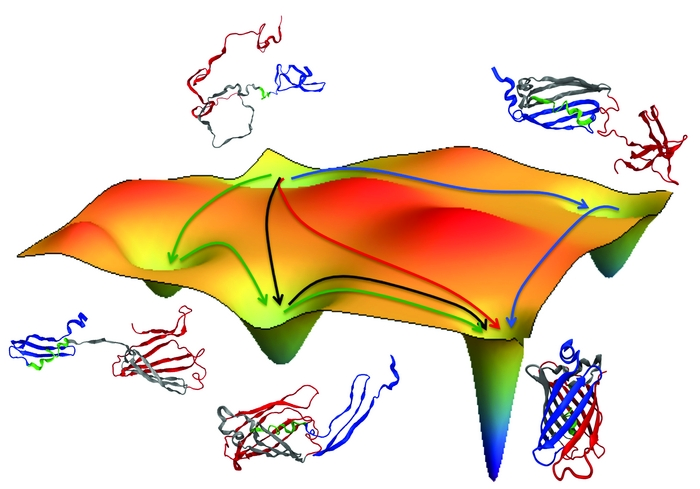
\includegraphics[width=1.0\linewidth]{images/ProteinFolding.png}
			       \caption*{Reddy, G.; Liu, Z.; Thirumalai, D. Proc. Natl. Acad. Sci. 2012, 109 (44), 17832–17838.}
			   \end{figure}
           \end{column}
       \end{columns}     
\end{frame}
}

{%
\setbeamertemplate{frame footer}{}
\begin{frame}[fragile]{The Problem}
    \begin{columns}{}
        \begin{column}{0.6\textwidth}
            \begin{itemize}
              \item[]<1->{
             	\metroset{block=fill}
             	\begin{block}{Computational methods require knowledge of molecular structure}
                    We need to find the lowest energy structure
             	\end{block}
              }
              \item[]<2->{
             	~
             	\metroset{block=fill}
             	\begin{block}{The potential energy surface (PES) is high dimensional and has many minima}
                    We can't tell for sure if we've found the \alert{\textbf{global}} minimum
             	\end{block}
              }
              \item[]<3->{
             	~
             	\metroset{block=fill}
            	\begin{block}{We may need information about one or more low-energy conformations}
                    \begin{itemize}[leftmargin=*]
                        \item<3-> Ok, let's find them all!
                        \item<4-> Under a cutoff
                    \end{itemize}
            	\end{block}
              }
            \end{itemize}
           \end{column}
           \begin{column}{0.45\textwidth}
		    \begin{overprint}
			    \onslide<2>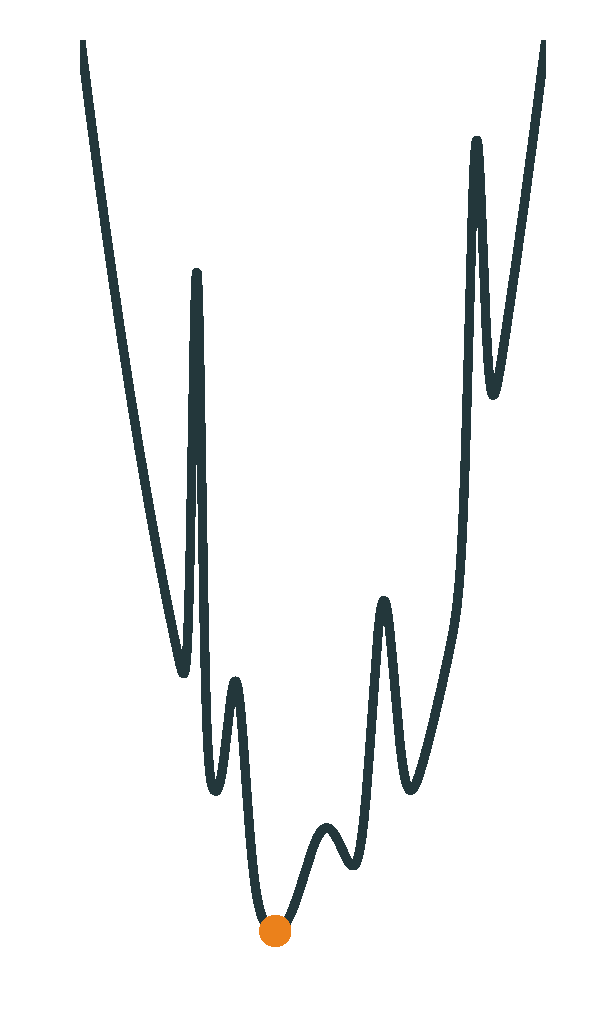
\includegraphics[width=0.9\linewidth]{images/globalmin.eps}
				\onslide<3>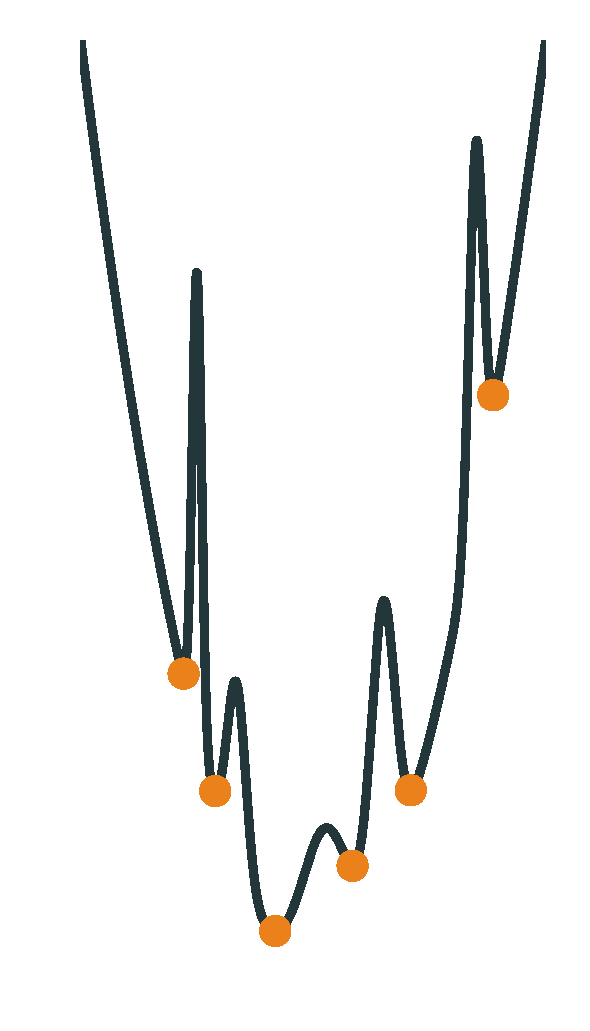
\includegraphics[width=0.9\linewidth]{images/manymins.eps}
				\onslide<4>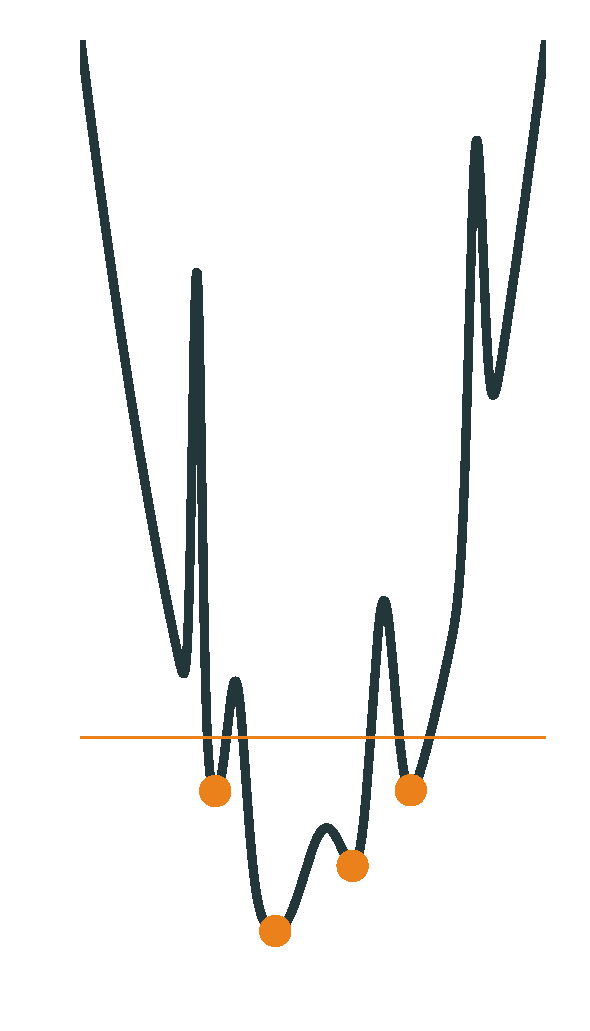
\includegraphics[width=0.9\linewidth]{images/cutoff.eps}
			\end{overprint}
           \end{column}
       \end{columns}     
\end{frame}
}
{%
\setbeamertemplate{frame footer}{Supady, A.; Blum, V.; Baldauf, C. J. Chem. Inf. Model. 2015, 55 (11), 2338–2348.}
\begin{frame}[fragile]{Possible Solutions}
	\begin{columns}[c] % align columns
		\begin{column}{.4\textwidth}
			\begin{itemize}[<+->]
				\item {Many techniques are well established}
				\item {None are perfect}
			\end{itemize}
		\end{column}
		\hfill
		\begin{column}{.65\textwidth}
			\footnotesize
			\begin{tabular}{ l  l}
				Method & Implented in
				\\ \midrule
				grid-based & CEASAR, \textbf{Open Babel, Confab,} \\
				           & MacroModel, MOE  \\
				rule-based & \textbf{ALFA, CONFECT,} CORINA, \\
				           & ROTATE, \textbf{COSMOS}, OMEGA \\
				population-based & \textbf{Balloon, Cyndi} \\
				basin-hopping & \textbf{ASE, GMIN, TINKER SCAN} \\
			\end{tabular}
		\end{column}
	\end{columns}
\end{frame}
}

\begin{frame}{Desirables}
	\metroset{block=fill}
	\begin{block}{What Algorithmic Properties do we want for conformer search?}
		\begin{itemize}[<+->]
			\item[1.] Accurate energies \& Structures
			\item[2.] {Minimize \# of geometry optimizations}
			\item[3.] {Find many low energy conformations}
			\item[4.] {Minimize human bias}
			\item[5.] {Parallel}
		\end{itemize}
	\end{block}
\end{frame}

\section{The Genetic Algorithm}

{%
	\setbeamertemplate{frame footer}{}
\begin{frame}{Outline}
	\begin{itemize}
		\item{At least 23 years
    		\begin{itemize}
        		\item[]{Judson, R. S.; Jaeger, E. P.; Treasurywala, A. M.; Peterson, M. L. J. Comput. Chem. 1993, 14 (11), 1407–1414.}
        	\end{itemize}
        }
		\item {Flexible ligand docking (Most cited: 7428) 
    		\begin{itemize}
        		\item[]{Morris, G. et al. J. Comput. Chem. 1998, 19 (14), 1639$–$1662.}
        	\end{itemize}
		}

   		\item{Precombustion CO${}_2$ adsorbing MOFs (October 14${}^{th}$)
       		\begin{itemize}
           		\item[]{Chung, Y. G.; Gomez-Gualdron, D. A.; Li, P.; Leperi, K. T.; Deria, P.; Zhang, H.; Vermeulen, N. A.; Stoddart, J. F.; You, F.; Hupp, J. T.; Farha, O. K.; Snurr, R. Q. Sci. Adv. 2016, 2 (10)}
           	\end{itemize}
        }
	\end{itemize}
\end{frame}
}

{%
	\setbeamertemplate{frame footer}{1. Carwright, H. Reviews in Computational Chemistry 2007 (25), pp 349$-$389.
}
\begin{frame}{Outline}
	\begin{columns}[c] % align columns
		\begin{column}{.48\textwidth}
			\begin{itemize}[<+->]
				\item {Inspired by biological evolution}
				\item {Evolve a population over generations}
				\item {Survival of the fittest}
				\item {Requirements:}
				\begin{itemize}
					\item {Represent individuals as vector}
					\item {Fitness function}
				\end{itemize}
				\item{$v = \left(\begin{smallmatrix}
					x_1 & y_1 & z_1 & x_2 &  y_2 & z_2 &
					\cdots & x_N & y_N & z_N
					\end{smallmatrix}\right)$}
				\item{$F = \frac{E_{\max} - E}{E_{\max} - E_{\min}}$}
			\end{itemize}

		\end{column}
		\hfill
		\begin{column}{0.48\textwidth}
			\begin{figure}
			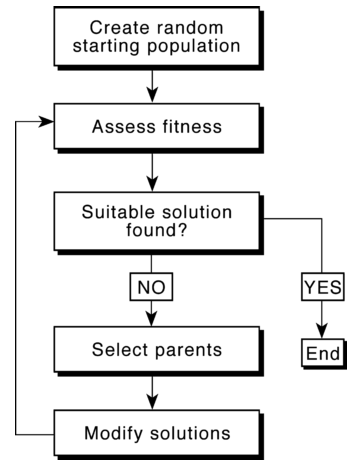
\includegraphics[width=0.8\linewidth]{images/GA_outline_Carwright.PNG}
			\end{figure}
		\end{column}
	\end{columns}
\end{frame}
}

{%
\setbeamertemplate{frame footer}{1. Supady, A.; Blum, V.; Baldauf, C. J. Chem. Inf. Model. 2015, 55 (11), 2338–2348.

2.~http://www.chemspider.com/Chemical-Structure.2298795.html}

\begin{frame}{The Many Representations of a Molecule}

  \begin{columns}[c] % align columns

    \begin{column}{.3\textwidth}
      \begin{itemize}
        \item[] {\alert{2D Image}}
        \item[] {
\includegraphics[width=0.95\linewidth]{images/2dRepr.PNG}}
        \item[] {\alert{3D Image}}
        \item[] {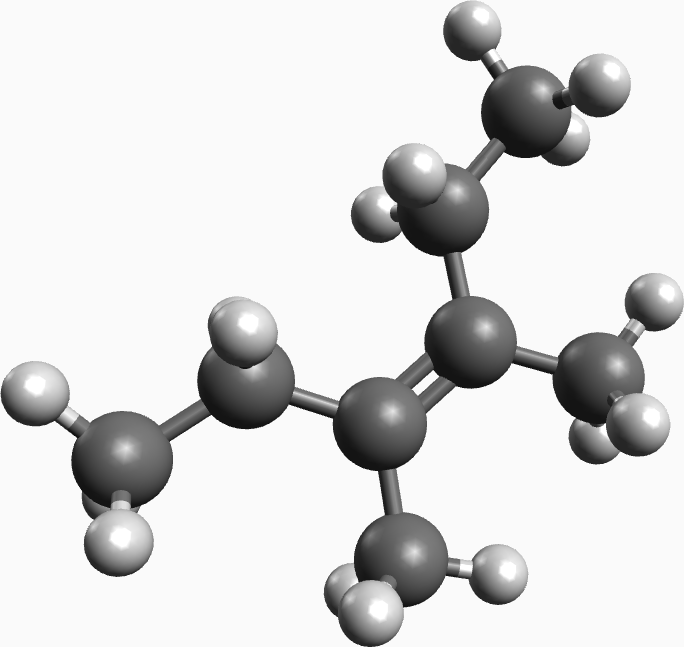
\includegraphics[width=0.95\linewidth]{images/3dRepr.PNG}}
      \end{itemize}
    \end{column}
        
    \begin{column}{0.3\textwidth}
      \begin{itemize}
		   \item[] {\alert{Name} \mbox{(3Z)-3,4-Dimethyl}-3-hexene}
		   \item[] {\alert{SMILES} CCC(C)=C(C)CC}
		   \item[] {\alert{InChI} 1S/C8H16/c1-5-7(3)8(4)6-2/h5-6H2,1-4H3/b8-7-}
      \end{itemize}
    \end{column}
   
    \begin{column}{0.45\textwidth}
        \begin{itemize}
      \item[] {\alert{Cartesian Coords}}
      \item[] {
        \begin{tabular}{l c c c}
              &         x    &       y     &      z  \\
          C   &       0.90   &    -0.25    &    0.02 \\
          C   &       2.35   &     0.15    &   -0.17 \\
          C   &       2.91   &     1.30    &   -0.67 \\
        \end{tabular}
        }
          \item[]{}
          \item[] {\alert{Internal Coords}}
          \item[] {
            \begin{tabular}{l c c c c}
              &   &   r  &   &  $\theta$ \\
            C &   &      &   &           \\
            C & 1 & 1.51 &   &           \\
            C & 2 & 1.38 & 1 & 131       \\
            \end{tabular}
          }
          \end{itemize}
    \end{column}
   
  \end{columns}
\alert{Internal Coords} are the natural choice here
\end{frame}

{%
\setbeamertemplate{frame footer}{}
\begin{frame}{Selecting Parents}
	\begin{columns}[c] % align columns
		\begin{column}{.48\textwidth}
			\metroset{block=fill}
			\begin{block}{Roulette Wheel Method}
    			\begin{itemize}[<+->]
    				\item[1.] {Reinforce good characteristics}
    				\item[2.] {Still give losers a chance}
    				\item[3.] {'Breed' pairs of winners}
    			\end{itemize}
			\end{block}
		\end{column}
		\hfill
		\begin{column}{0.48\textwidth}
		    \begin{overprint}
			    \onslide<4>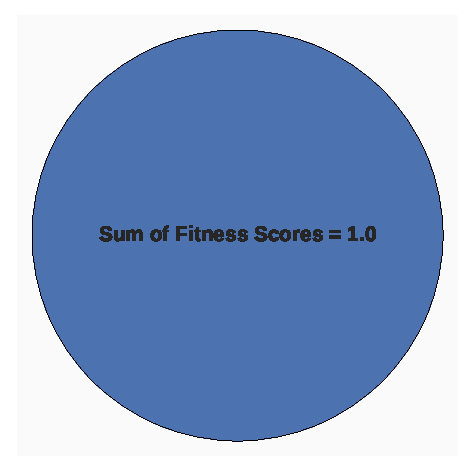
\includegraphics[width=\linewidth]{images/pie0.eps}
				\onslide<5>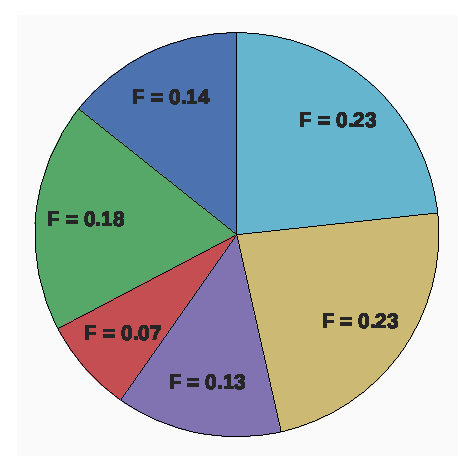
\includegraphics[width=\linewidth]{images/pie1.eps}
				\onslide<6>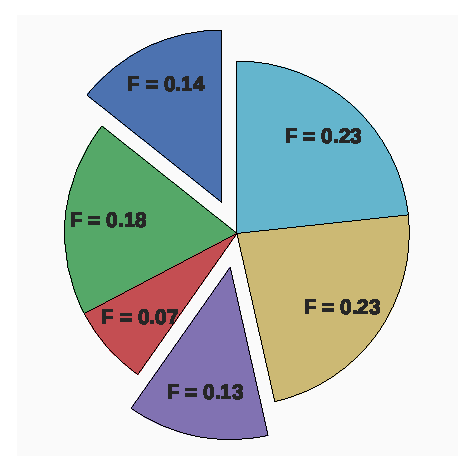
\includegraphics[width=1.1\linewidth]{images/pie2.eps}
			\end{overprint}
		\end{column}
	\end{columns}
\end{frame}

{%
\setbeamertemplate{frame footer}{}
\begin{frame}{The Next Generation}
    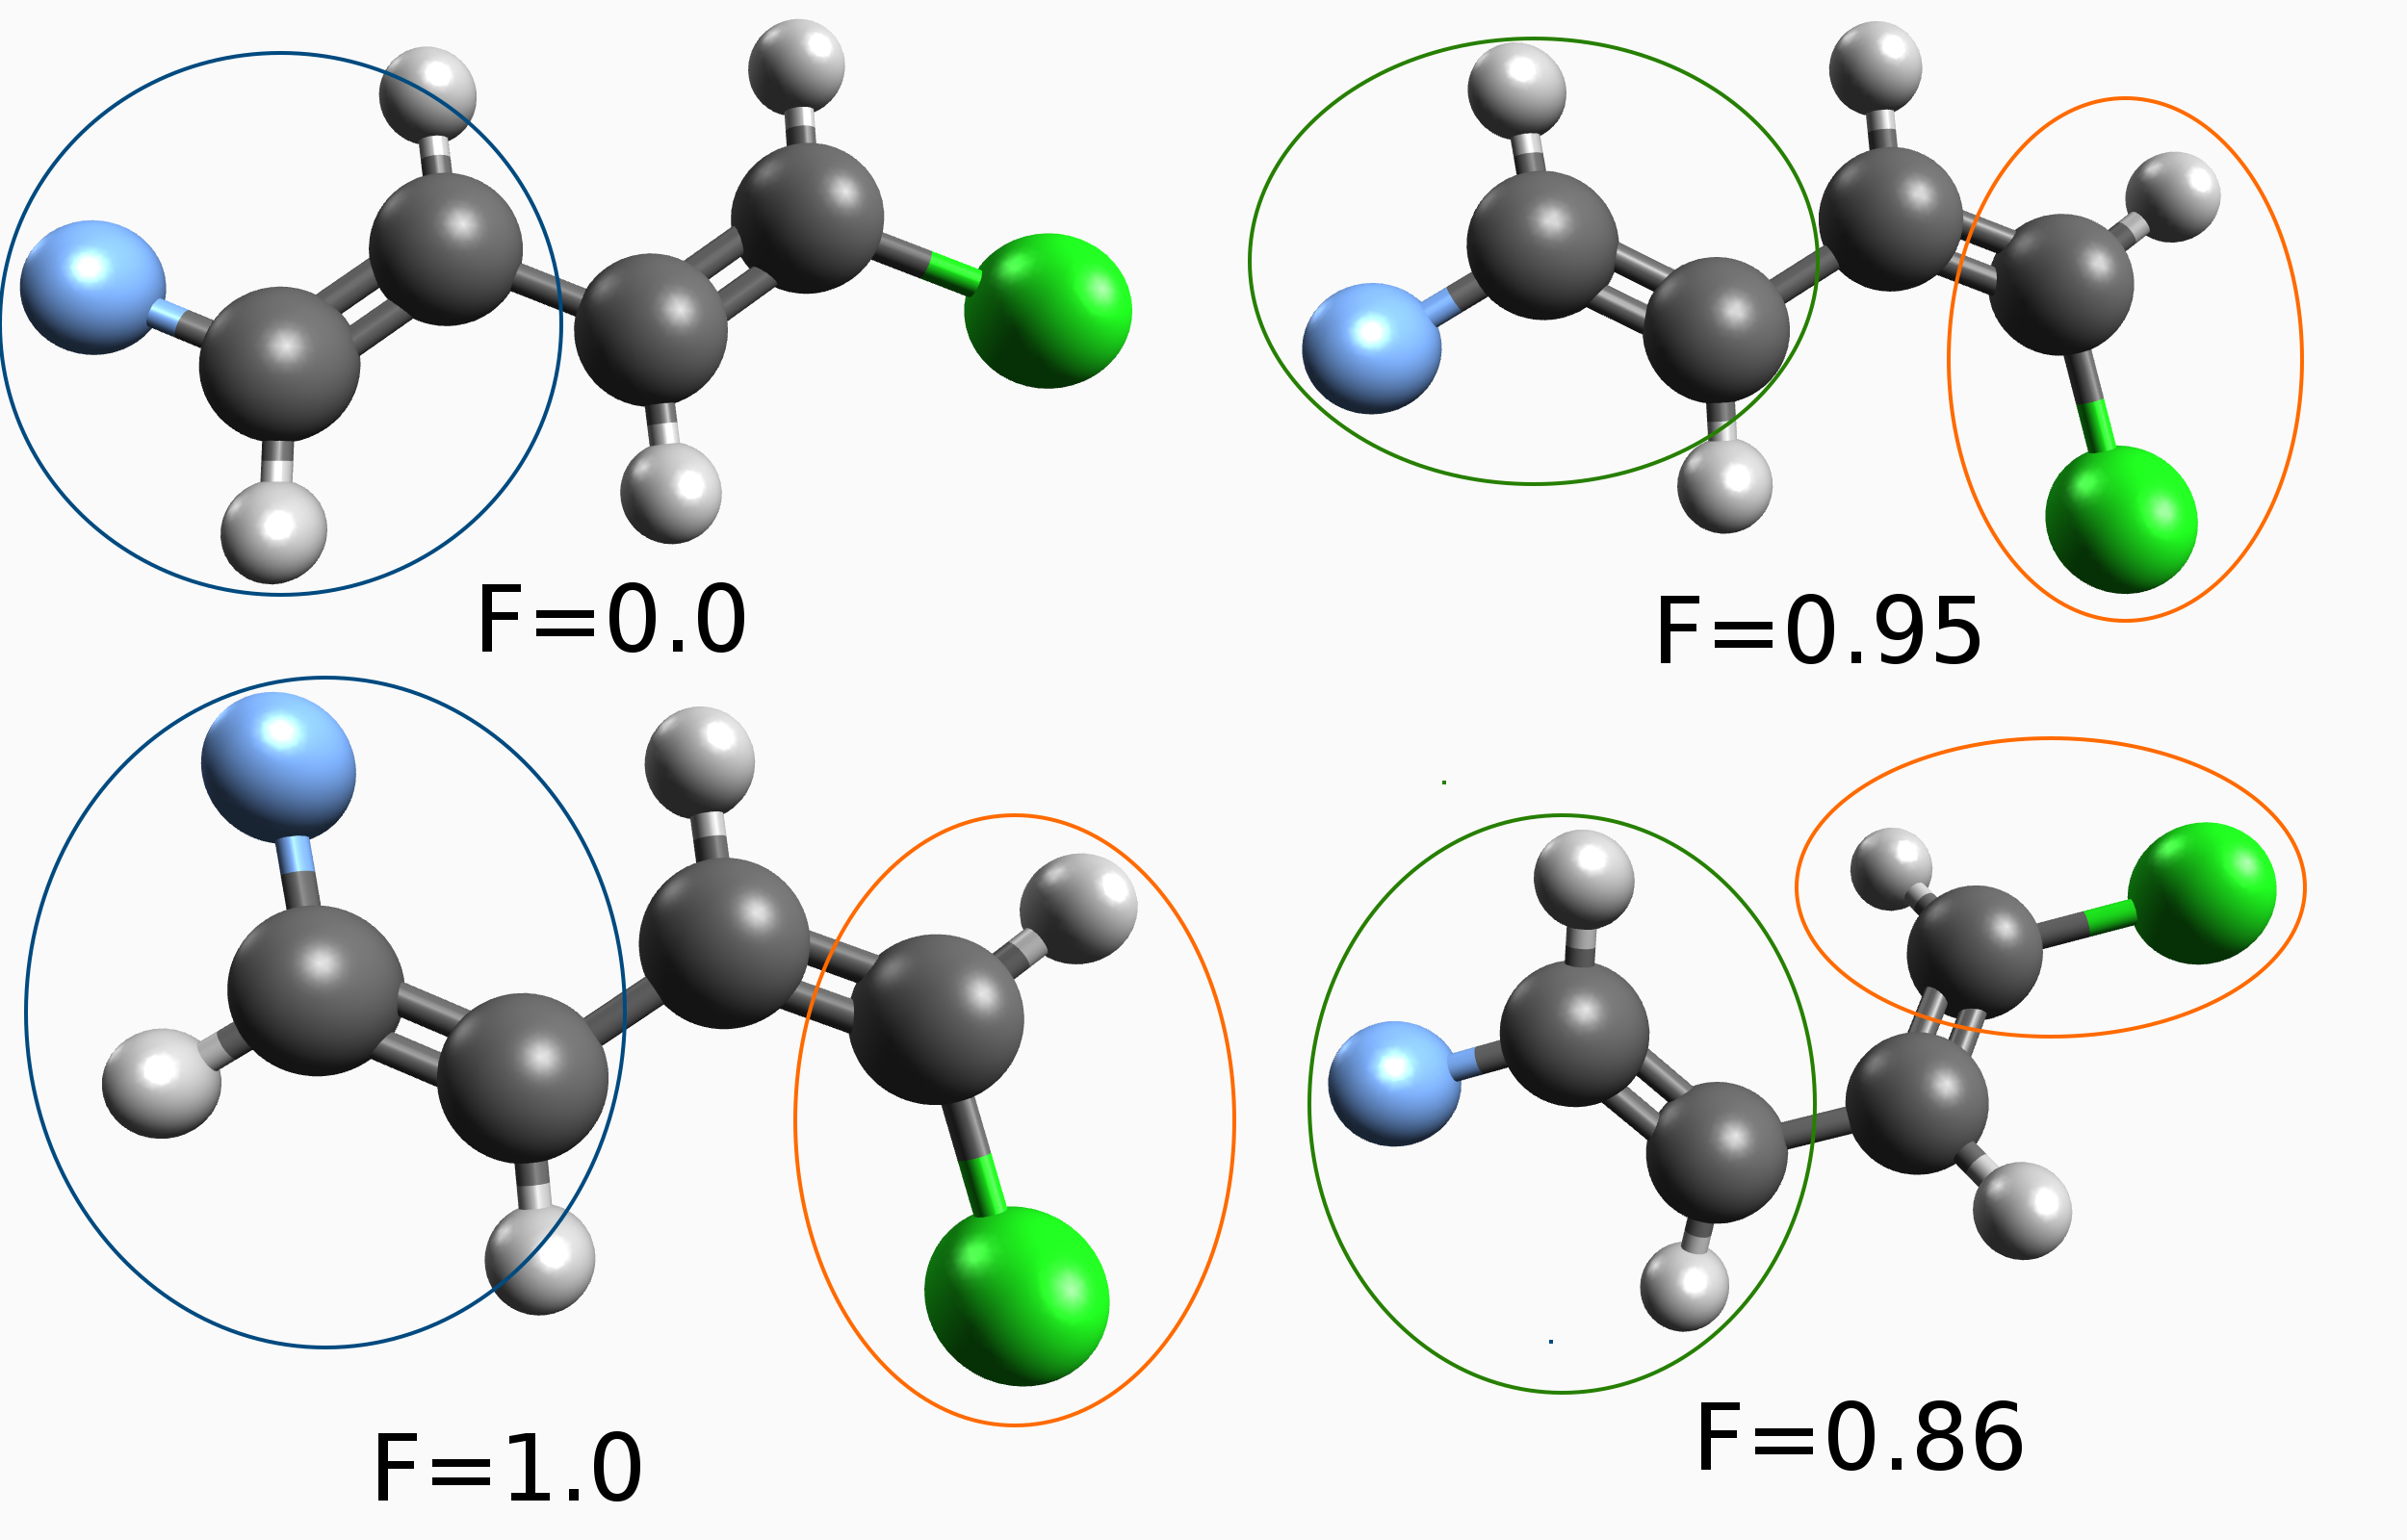
\includegraphics[width=\linewidth]{images/nextgen.png}
\end{frame}
}


\begin{frame}{The Whole Algorithm}
	\begin{columns}[c] % align columns
		\begin{column}{.5\textwidth}
			\begin{itemize}
				\item[1.]<1-> {Generate N random, sensible geometries}
				\item[2.]<3-> {Optimize}
				\item[3.]<4-> {Select Parents}
				\item[4.]<5-> {Crossover \& Mutate}
				\item[5.]<6-> {Add Children to population}
				\item[6.]<7-> {Remove the unfit}
				\item[7.]<8-> {If converged:
    				\begin{itemize}
    					\item{Done!}
    				\end{itemize}
				}
				\item[]<9-> {Otherwise:
    				\begin{itemize}
    					\item{Go to 2}
    				\end{itemize}
				}
			\end{itemize}
		\end{column}
		\hfill
		\begin{column}{0.6\textwidth}
			\begin{itemize}
				\medskip
				\uncover<1->{
				\item[]{
					\begin{figure}
						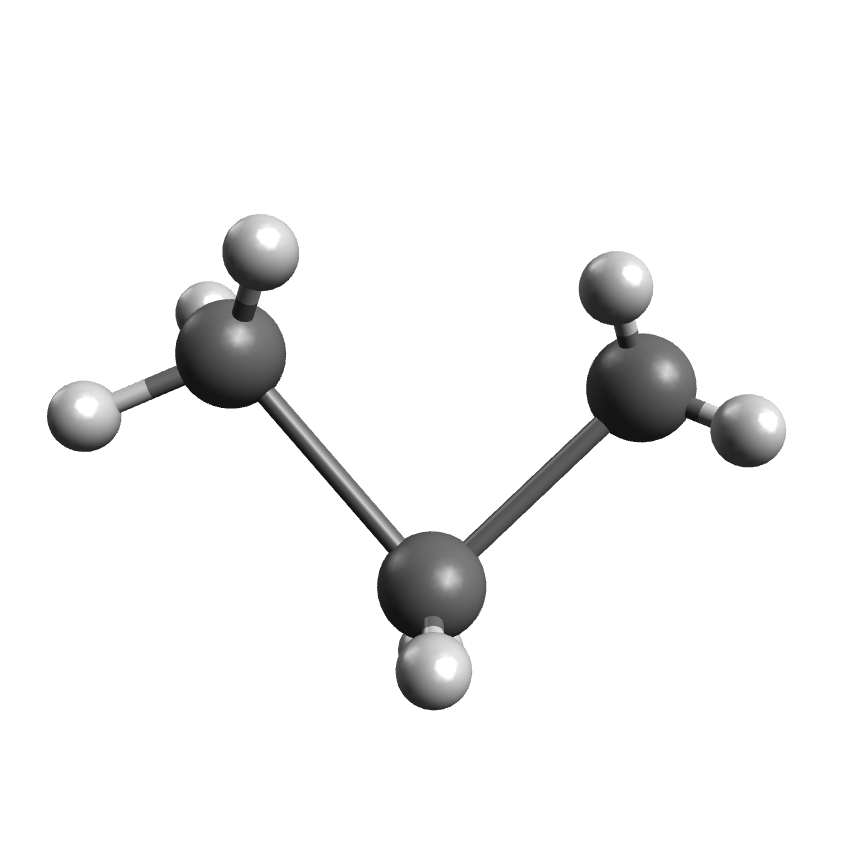
\includegraphics[width=0.6\linewidth]{images/sense.png}
						\caption*{sensible}
					\end{figure}
				}}
				\uncover<2->{
			    \item[]{
			    	\begin{figure}
					    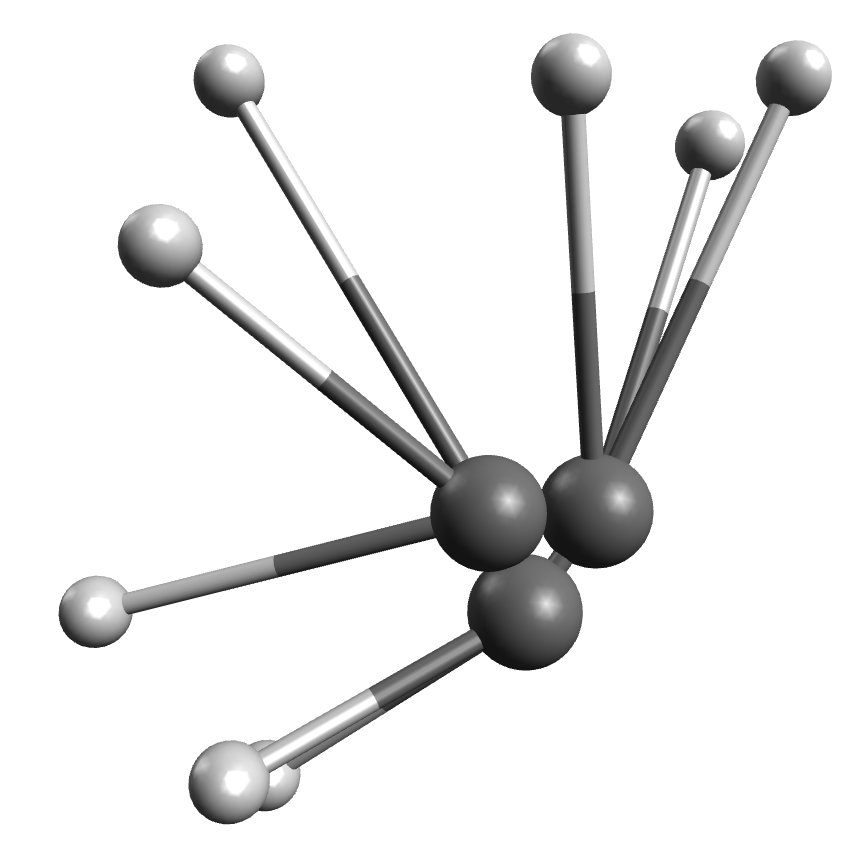
\includegraphics[width=0.4\linewidth]{images/nonsense.png}
					    \caption*{utter nonsense}
					\end{figure}
				}}
			\end{itemize}
		\end{column}
	\end{columns}
	~
\end{frame}

\section{Finding Low Energy Conformers of Dipeptides}

{%
	\setbeamertemplate{frame footer}{Supady, A.; Blum, V.; Baldauf, C. J. Chem. Inf. Model. 2015, 55 (11), 2338–2348.}
\begin{frame}{"Dipeptide" Structures}
   	\begin{figure}
   		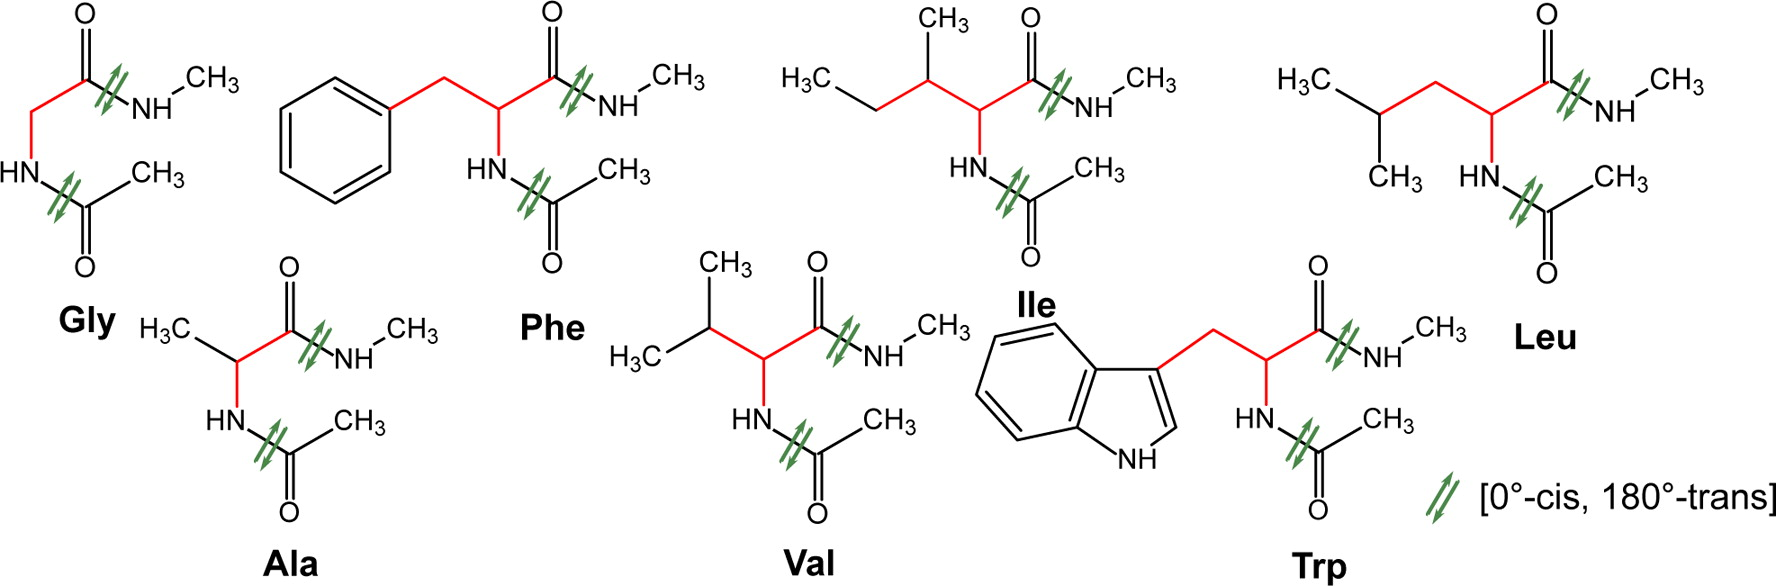
\includegraphics[width=\linewidth]{images/Supady2.png}
   		\caption*{\textcolor{red}{Red} = Rotatable bonds \\
		   		  \textbf{\textcolor{darkgreen}{\ce{<=>}}} = Cis/Trans Bonds
		   		  }
   	\end{figure}
   	\begin{quote}
       	"We use the term dipeptide for amino acids with an acetylated 
       	N terminus and an amino-methylated C terminus"
    \end{quote}
\end{frame}
}

{%
\setbeamertemplate{frame footer}{Supady, A.; Blum, V.; Baldauf, C. J. Chem. Inf. Model. 2015, 55 (11), 2338–2348.
}
\begin{frame}{Combinatorics}
	\begin{columns}[c] % align columns
		\begin{column}{.3\textwidth}
			\begin{itemize}
				\item {GA beats other methods if space is large}
				\item {Space gets large \textbf{\alert{fast}}}
			\end{itemize}
		\end{column}
		\hfill
		\begin{column}{0.8\textwidth}
			%\begin{figure}
			%	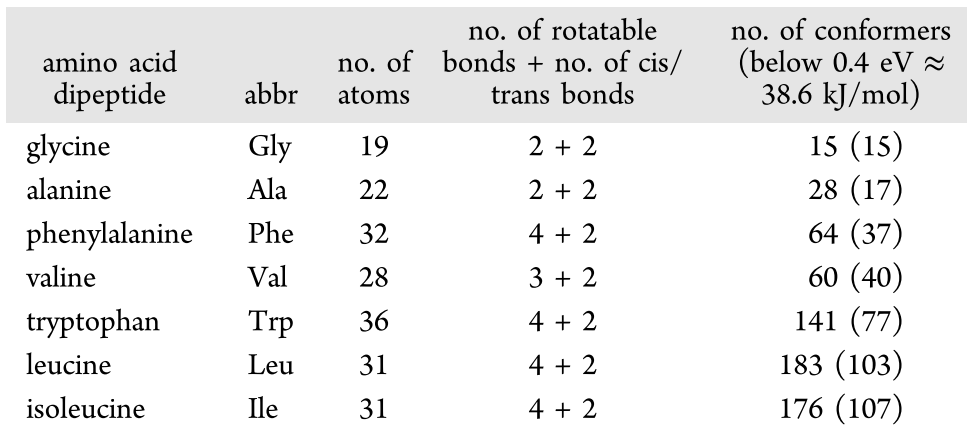
\includegraphics[width=\linewidth]{images/Confnums.png}	
			%\end{figure}
            \begin{tabular}{l c c c r}
                     &    & \# Rotatable +     &               \\
            Molecule & N  & \# Cis/Trans Bonds & \# Conformers \\
            \midrule
            Gly & 19 & 2 + 2 & 15  \\
            Ala & 22 & 2 + 2 & 28  \\
            Phe & 32 & 4 + 2 & 64  \\
            Val & 28 & 3 + 2 & 60  \\
            Trp & 36 & 4 + 2 & 141 \\
            Leu & 31 & 4 + 2 & 183 \\
            Ile & 31 & 4 + 2 & 176 \\
            \end{tabular}
		\end{column}
	\end{columns}
\end{frame}
}

{%
\setbeamertemplate{frame footer}{1) Supady, A.; Blum, V.; Baldauf, C. J. Chem. Inf. Model. 2015, 55 (11), 2338–2348.

2) Ropo, M.; Schneider, M.; Baldauf, C.; Blum, V. Sci. Data 2016, 3, 160009.
}
\begin{frame}{Coverage}
	\begin{columns}[c] % align columns
		\begin{column}{.4\textwidth}
			\begin{itemize}
				\item {Smaller systems are reliably sampled}
				\item {As \# of conformers increases, miss more and more}
				\item {Is there a pattern to what is missed?}
			\end{itemize}
		\end{column}
		\hfill
		\begin{column}{0.6\textwidth}
			\begin{figure}
				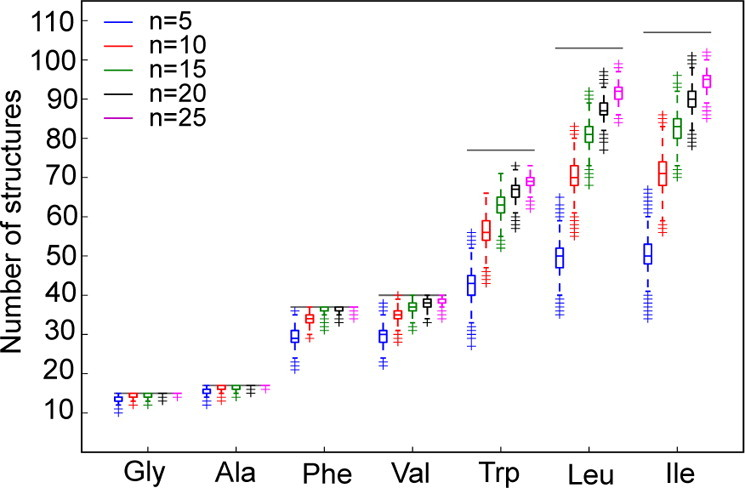
\includegraphics[width=\linewidth]{images/Supady4.png}
				\caption*{Proportion of conformers found with increasing runs of the GA}
			\end{figure}
		\end{column}
	\end{columns}
\end{frame}
}

{%
\setbeamertemplate{frame footer}{Supady, A.; Blum, V.; Baldauf, C. J. Chem. Inf. Model. 2015, 55 (11), 2338–2348.
}
\begin{frame}{Coverage}
	\begin{columns}[c] % align columns
		\begin{column}{.4\textwidth}
			\begin{itemize}[<+->]
				\item {Most misses are very high energy}
				\item {Algorithm favors low energy areas of the space}
				\item {Features low in energy are favored and recombined}
			\end{itemize}
		\end{column}
		\hfill
		\begin{column}{0.6\textwidth}
			\begin{figure}
				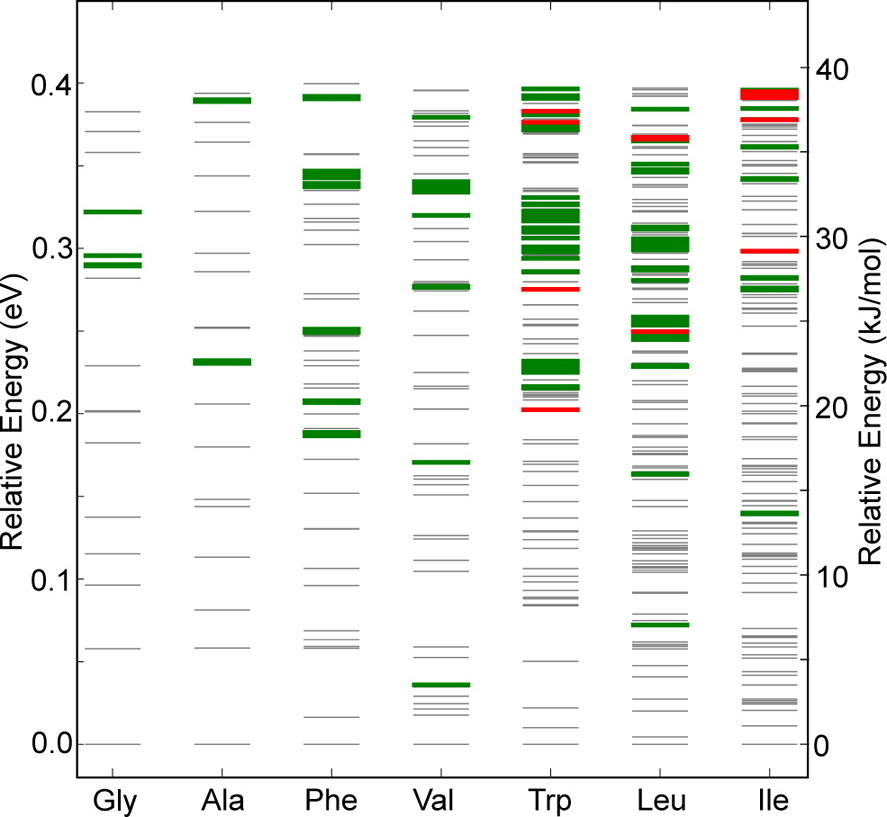
\includegraphics[width=0.75\linewidth]{images/Supady5.png}
				\caption*{\textcolor{red}{---} Missed by the GA \\
				  \textcolor{darkgreen}{---} New Found by GA \\
				  \textcolor{gray}{---} In Reference \& GA}
			\end{figure}
		\end{column}
	\end{columns}
\end{frame}
}

{%
\setbeamertemplate{frame footer}{Supady, A.; Blum, V.; Baldauf, C. J. Chem. Inf. Model. 2015, 55 (11), 2338–2348.}
\begin{frame}{Energy Cutoff}
	\begin{columns}[c] % align columns
		\begin{column}{.4\textwidth}
			\begin{itemize}[<+->]
				\item[] {
					\begin{figure}
					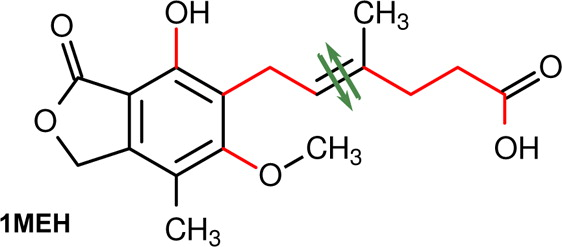
\includegraphics[width=\linewidth]{images/Supady3.png}
					\caption*{Mycophenolic Acid}
					\end{figure}
				}
				\item {GA is more sensitive to energy cutoff}
				\item {For finding low energy ensemble, GA outperforms purely stochastic/deterministic method}
			\end{itemize}
		\end{column}
		\hfill
		\begin{column}{0.6\textwidth}
			\begin{figure}
				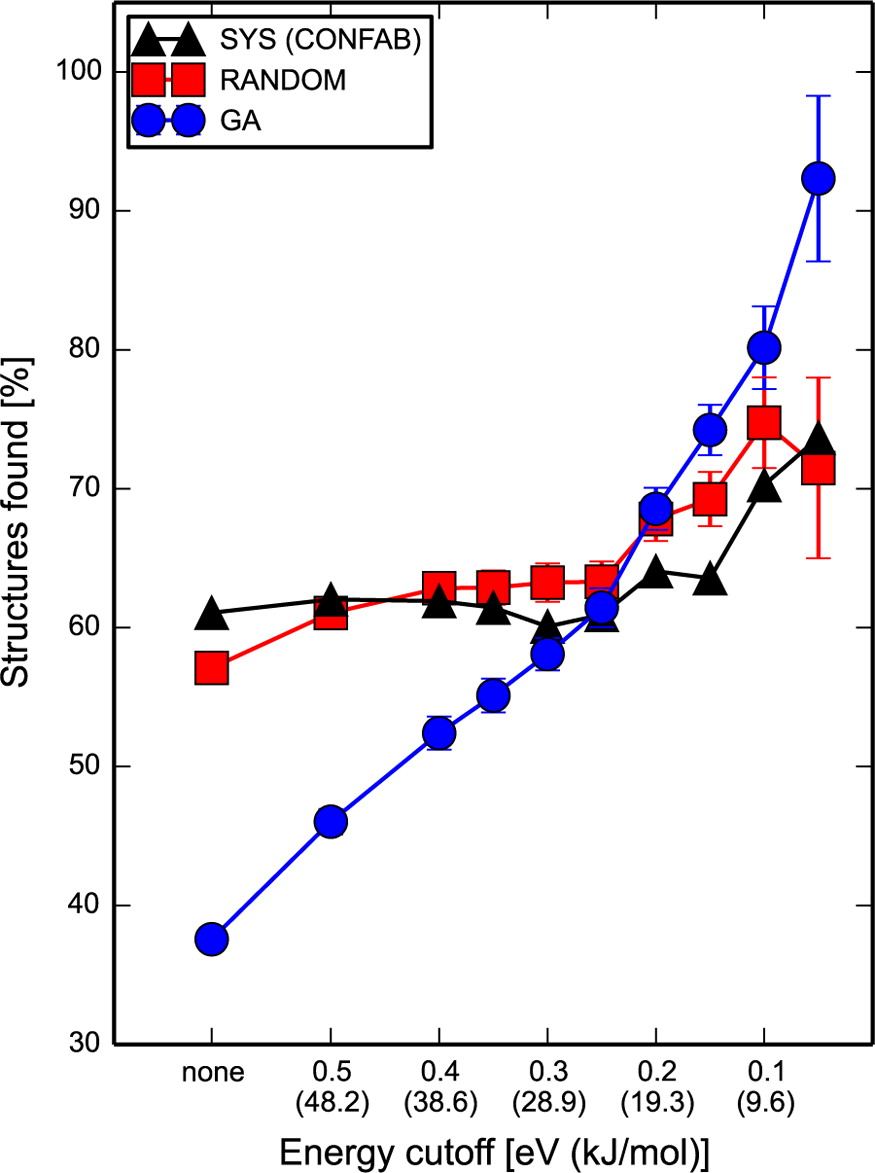
\includegraphics[width=0.75\linewidth]{images/Supady6.png}
				%\caption*{\textcolor{red}{a}}
			\end{figure}
		\end{column}
	\end{columns}
\end{frame}
}

\section{Concluding Remarks}

{%
\setbeamertemplate{frame footer}{Supady, A.; Blum, V.; Baldauf, C. J. Chem. Inf. Model. 2015, 55 (11), 2338–2348.}
\begin{frame}{Concluding Remarks}
    \metroset{block=fill}
    \begin{block}{Review}
    	\begin{itemize}[<+->]
    		\item {Conformational searching is expensive}
    		\item {The Genetic Algorithm is a guided global search}
    		\item {It shines when asked to find many low energy solutions}
    		\item {GA can be used with any electronic structure package}
    		\item {This one is available under the GNU Lesser General Public License:
            		\url{https://github.com/adrianasupady/fafoom}}
    	\end{itemize}
    \end{block}
\end{frame}
}


\begin{frame}[standout]
  Questions?
\end{frame}

\appendix

\begin{frame}[fragile]{Backup slide}
	\begin{itemize}
		\item Geometry optimization step makes the algorithm more Lamarckian (Jean Baptiste Larmarck, [1744-1829])
	\end{itemize}
\end{frame}

{%
\setbeamertemplate{frame footer}{(1) Blum, V. et.`\' al., M. Comput. Phys. Commun. 2009, 180 (11), 2175–2196.

(2) Supady, A.; Blum, V.; Baldauf, C. J. Chem. Inf. Model. 2015, 55 (11), 2338–2348.

	}
\begin{frame}[fragile]{Genetic Algorithm Parameters}
	Geometry Optimization: DFT PBE + VdW, \emph{tier1} basis in FHI-aims$^1$.
	Convergence at 0.005 eV /\AA{}
	\begin{figure}
		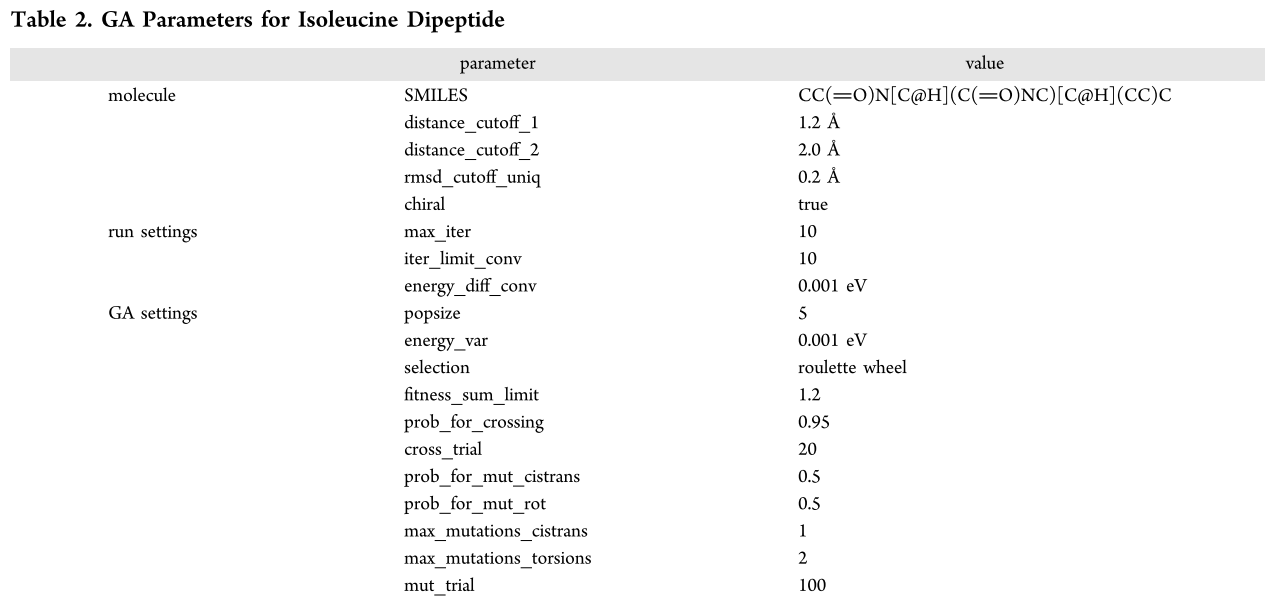
\includegraphics[width=\linewidth, trim={0 0 0 1.2cm},clip]{images/Params.png}
		\caption*{GA Parameters for Isoleucine Dipeptide$^2$}
	\end{figure}
\end{frame}
}
\end{document}
